\documentclass[UTF8,12pt]{article}
\usepackage[colorlinks,linkcolor=black]{hyperref}
\usepackage{longtable}
\usepackage{xcolor}
\usepackage{colortbl}
\usepackage{mathtools}
\usepackage{multirow}
\usepackage{amsmath,bm}
\usepackage{amssymb}
\usepackage{float}
\usepackage{ctex}
\usepackage{appendix}
\usepackage{graphicx}
\usepackage{caption}
\usepackage{subcaption}
\usepackage{listings}
\usepackage[a4paper,left=10mm,right=10mm,top=15mm,bottom=15mm]{geometry}
\graphicspath{{Pic/}} 	% 在于.tex同级的目录下创建名为pic的文件夹,存放图片
\title{对比特币矿池的DoS攻击}
\date{}
\author{18308045 谷正阳}
\begin{document}
\maketitle
\section{DoS攻击}
\subsection{简介}
DoS攻击即拒绝服务攻击,是一种用于破坏用户合法访问目标网络和网络资源的攻击。一般来说,它是通过用大量的流量或恶意请求令目标(网络服务器通常是网络服务器)过载,使目标服务器故障甚至完全
失灵。首例有记载的DoS攻击发生于2000年2月,由一个15岁的加拿大黑客对Amazon和eBay的网络服务器发起。自此以后,越来越多的人利用DoS攻击来破坏许多行业的目标。
\subsection{种类}
由于不是所有的设备和网络都易受同一种方法的危害,那些造成危害的攻击经常是可以巧妙地运用漏洞进行。以下是几种常见的DoS攻击种类。
\subsubsection{缓冲区溢出攻击}
缓冲区溢出攻击是最常用的攻击,它通过发送比目标设计能够处理流量更多的流量来实现。这种攻击可以使目标进程崩溃。
\subsubsection{ICMP flood攻击}
ICMP flood攻击在目标网络错误地配置一台设备,强制其对每个节点发送伪造包,使网络过载。
\subsubsection{SYN flood攻击}
SYN flood攻击发送请求连接目标网络服务器,但不完成完整的连接认证,然后继续对目标的每个剩余的开放的端口重复上述操作直至致使目标服务器崩溃。
\subsection{区块链对BDoS攻击的防御机制}
\subsubsection{去中心化}
区块链的去中心化机制为其抵御DoS攻击和DDoS攻击提供了强大的支撑。即使是许多节点无法通信或下线,整个区块链仍可以继续运行并验证交易。当那些崩溃的节点可以重新恢复工作时,它们又可以重新同步
并获得那些没受攻击的节点提供的数据,重新跟上最近的数据进度。区块链可以抵御这些攻击的程度与网络的节点数和哈希率有关,对于最老最大的加密货币比特币而言,它被认为是最安全且最不易受攻击的
区块链。这意味着DoS攻击和DDoS攻击更不容易对其造成崩溃。
\subsubsection{工作量证明}
工作量证明机制使得对比特币的许多攻击十分昂贵。矿工只能证明他们在系统外花费了计算能力来创建区块。仅当系统中的大部分计算能力运行正常时,才能维护区块链的安全。因此,攻击者要进行攻击,
其拥有的计算能力就要比其他参与者的总和都要高,即51\%攻击。对于主要的加密货币来说,51\%攻击的代价对于大多数实体而言都是难以承担的。
\section{对比特币矿池的DoS攻击}
\subsection{比特币矿池}
由于比特币全网的运算水准在不断的呈指数级别上涨,单个算力微弱的矿工难以获得收益,于是就出现了多个矿工联合算力挖矿,挖出的比特币奖励按贡献度分享,这便是矿池。大多数矿池都是“托管矿池”,
即公司或者个人运营着矿池服务器。矿池服务器运行着专用的软件,根据矿池挖矿协议来协调矿工们的工作。其他机器自然知道其公网ip及开放端口,可以利用此来进行SYN flood攻击令矿池服务器瘫痪进而
达到攻击整个矿池的目的。
\subsection{具体实现}
TCP协议是进程与进程之间建立,要建立连接,会先进行三次握手:
\begin{figure}[H]
    \centering
    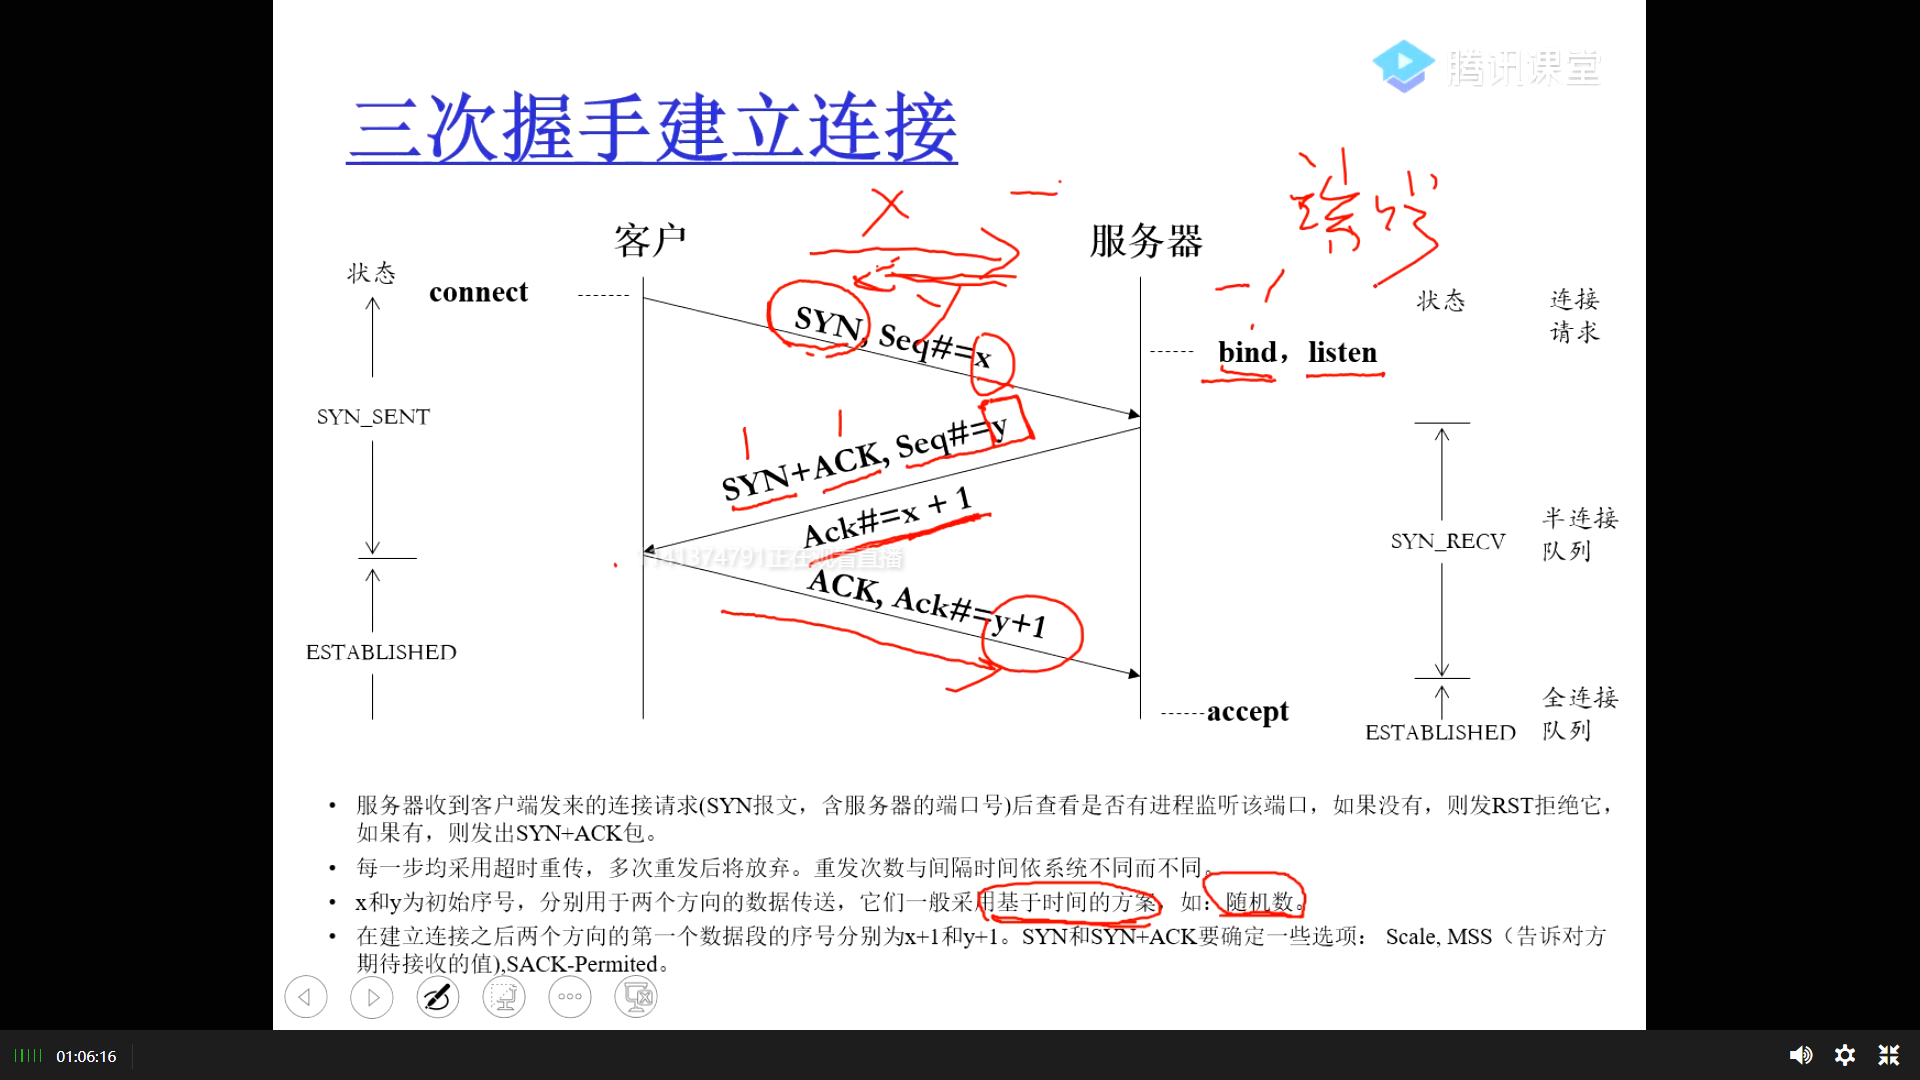
\includegraphics[width = \textwidth]{shaking.png}
\end{figure}
而这个流程有一个缺陷:在第二次握手在接受服务器发送的SYN+ACK报文后不发送ACK,服务器会等待对方放入半连接队列,并等待ACK,超时重传SYN+ACK,直至超过重复次数才会释放连接。默认重试次数为
5次,重试的间隔时间从1s开始每次都番倍,分别为1s + 2s + 4s + 8s +16s = 31s,第5次发出后还要等32s才知道第5次也超时了,所以一共是31 + 32 = 63s。这个时间非常长。另外由于半连接队列
是有长度限制的,默认是1024,如果攻击者在这个时间内不断对目标服务器开放的端口发送SYN报文,且收到SYN+ACK后不发送ACK。这样服务器的半连接队列会被大量占用以至占满,这样就无法再处理新的
连接请求也就无法继续协调矿工工作,这样整个矿池就崩溃了。

\section{对基于PBFT共识的区块链的DoS攻击}
上述方法是对矿池进行攻击,而对整个比特币社区,这种攻击无法奏效,因为整个社区是去中心化的,没有中心服务器。想要成功需要针对比特币社区的漏洞来进行特别的攻击。在区块链中,奖励机制促使矿工
挖矿,但是一旦激励机制不能够促进良好行为时,区块链就会处于危险之中。BDoS攻击就是利用这一点,会使得整个网络处于一种状态,使得理性矿工最佳的行动是停止挖掘。
\subsection{具体实现}
攻击者挖出一个块,然后只公布区块头。这时候矿工有三个选择:其可以延长主链,然后忽略区块头;其可以扩展这个区块头(SPV挖矿);其可以停止挖矿,既不消耗算力,也不赢得奖励。
\begin{figure}[H]
    \centering
    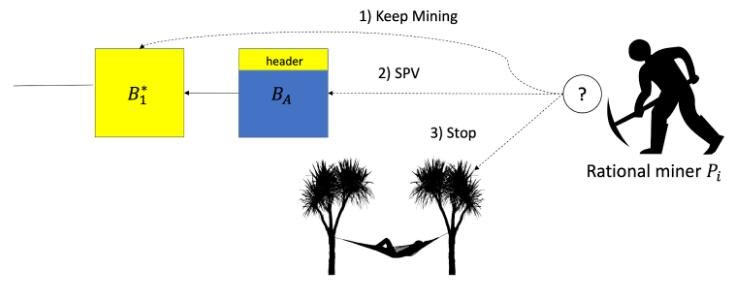
\includegraphics[width = 0.8 \textwidth]{choices.jpg}
\end{figure}
如果理性矿工选择扩展主链,找到并广播一个新的区块,那么攻击者矿工将那么攻击者就快速广播与区块头对应的完整块(攻击块)。因为点对点网络里每个节点的网络连通性不一致,有的节点会先收到
攻击块,有的节点会先收到防守块,这会导致两组矿工之间的竞争。
\begin{figure}[H]
    \centering
    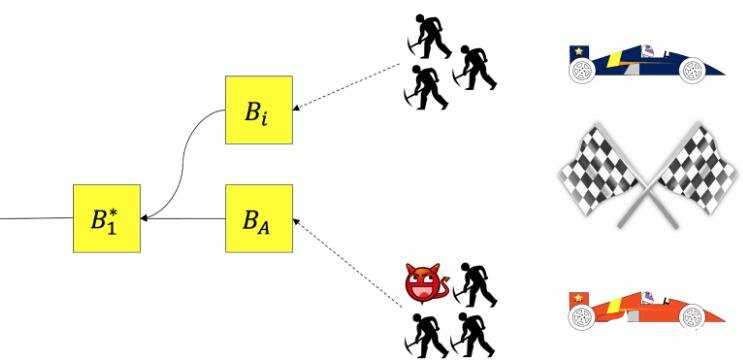
\includegraphics[width = 0.8 \textwidth]{compete.jpg}
\end{figure}
在一定概率下,该理性矿工会输掉比赛,使得区块Bi最终不被包含在主链当中。因而这种情况下在最后一个完整区块上挖矿的预期回报会低于一般情况。如果理性矿工遵循选择扩展这个区块头BA,则攻击者
就不会发布完整的区块BA。这导致这个区块不会上主链,从而导致该区块的预期回报为零。由于挖矿还需付出大量计算,一定情况下关机不继续挖矿成为预期净回报最高的选择,因而就使得奖励机制无法鼓励
矿工继续挖矿,进而无人记录交易,进而使整个网络瘫痪。
\subsection{影响}
\subsubsection{规则的共识}
规则即确保交易、区块有效的机制,保证了比特币参与者能够进行最基本的交互。而BDoS攻击可能会破坏奖励机制,导致理性的矿工最优的策略是不挖矿,这样相当于破坏了规则共识的一环。
\subsubsection{历史记录的共识}
记录即已发生的被记录在区块链串接的Merkle Tree上的交易,保证了去中心化的UTXO的正常运行。规则中如最长链原则,大家优先相信最长的账本,因而规则的共识促成了历史记录的共识。而BDoS攻击
一旦破坏规则共识,没有人继续挖矿或保有账本,因而也破坏了交易记录的分布式存储的一致性,导致破坏了历史纪录的共识。
\subsubsection{比特币价值的共识}
价值共识即与现实货币的汇率,保证所有人想要比特币,所有人可以用比特币交易。历史纪录的共识保证了人们对比特币的信任。然而BDoS一旦破坏了历史纪录的共识,会令人们丧失对比特币的信任,进而
降低对比特币的购买意愿,进而比特币贬值,又会导致一部分人抛售比特币,进而加速了比特币的贬值,最终破坏了比特币价值的共识。
\end{document}
